\chapter{Introduction}

This board allows to connect FPix modules (Phase-I upgrade) using a flex cable to connect it to the DTB. Its key features are:
\begin{itemize}
    \item Make the proper electrical connections between the TBM of the module and the DTB. This includes matching the impedances.
    \item Provide pass-through for the supply voltages to power the module.
    \item Provide a resistor bridge for measuring the temperature of the HDI using its RTD and two ADC channels in the DTB.
    \item Has an 2\,kbit EEPROM to identify the type of adapter, connected to the DTB via its \isqc{} bus.
    \item Can be mounted on a PSI cold box in a configuration of four boards.
    \item Displays the power on state on the board using an LED, selectable by a jumper
\end{itemize}

The following conventions are used throughout this document:
\begin{itemize}
    \item SCSI-connector: this refers to the 68-pin connector, which will be used to connect the adapter to the DTB.
    \item SMK-connector: this is a 2$\times$20 pin connector to connect to the FPix module using standard FPix flex cables.
    \item GND: ground.
    \item HV: High voltage, routed through the DTB and supplied by an external power supply.
    \item VA: Supply voltage for analog circuits in the ROC.
    \item VD: Supply voltage for digital circuits in the TBM and ROC.
    \item 3V3: 3.3\,V supply for support circuits.
    \item TBM: Token bit manager, custom ASIC on the HDI
    \item HDI: High-density interconnect, custom circuit on modules, makes connections between TBM and ROC
    \item ROC: Read-out chip
    \item DTB: Digital test board
\end{itemize}
This document is not a full documentation of the whole chain. Please refer to the specific documents about other parts. Most of this documentation can be found via \url{https://twiki.cern.ch/twiki/bin/viewauth/CMS/Psi46}

\section{Change log}
\begin{tabular}{cc}
    \toprule
    Version of this document & Version of the board \\
    \midrule
    0.0 & 1.1 \\
    1.0 & 2.0 \\
    \bottomrule
\end{tabular}

\bigskip

Changes to version 2.0 of module:
\begin{itemize}
    \item Removed signal networks for \texttt{RClk\_Out} and \texttt{160MHz\_Out}. The latter is no longer present in TBM chips after version 7, the return clock is not needed.
    \item Signals reshuffled on cable between module and adapter (consequence of previous change). This renders v2.0 of board \textbf{incompatible} to old versions of the HDI. In fact, operating an old HDI using a new adapter or vice versa shorts \texttt{VA} and \texttt{VD} shorted to \texttt{GND} and should be avoided.
    \item The impedance matching for the two signals from the module (\texttt{OutA} and \texttt{RDa}) has been adjusted to reduce the attenuation. Downside: impedance matching no longer symmetric but reflections are ok.
    \item Added an LED to display power status (otherwise only visible on back of DTB). For operation in a dark environment, this can be turned off removing a jumper.
    \item Adjusted impedance matching networks to match needs.
    \item Swap inner two layers (done at order).
    \item The 3.3\,V net is now fused on the board to prevent overcurrent in case of a short downstream the SCSI connector.
\end{itemize}

\chapter{Design considerations}
The board has been designed as a 4-layer PCB with the following topology:
\begin{center}
\begin{tabular}{cc}
	\toprule %-------------------------------------------------------------------------------------------------
Layer & Description \\
	\midrule %-------------------------------------------------------------------------------------------------
Top & Main signal layer \\
2nd & GND plane \\
3rd & Power plane, distributes \emph{VA}, \emph{VD}, and \emph{HV} \\
Bottom & Remaining signals \\
	\bottomrule %-------------------------------------------------------------------------------------------------
\end{tabular}
\end{center}

\section{Signal routing}

The signal connections between the TBM and the DTB are as follows:
\begin{center}
\begin{tabular}{lcll}
    \toprule %-------------------------------------------------------------------------------------------------
    TBM & direction & DTB & Comments \\
    \midrule %-------------------------------------------------------------------------------------------------
    \texttt{OutA}        & $\rightarrow$ & \texttt{SDATA1} & \\
    \texttt{RDa\_Out}    & $\rightarrow$ & \texttt{TOUT}   & \\
    \texttt{SD\_In}      & $\leftarrow$  & \texttt{SDA}    & \\
    \texttt{Trig\_In}    & $\leftarrow$  & \texttt{CTR}    & \\
    \texttt{Clk\_In}     & $\leftarrow$  & \texttt{CLK}    & \\
    \bottomrule %-------------------------------------------------------------------------------------------------
\end{tabular}
\end{center}

\section{Impedance matching of TBM signals}

The impedances of the two outer connections are not the same:
\begin{center}
\begin{tabular}{lc}
    \toprule %-------------------------------------------------------------------------------------------------
    Connection & Impedance $Z$ \\
    \midrule %-------------------------------------------------------------------------------------------------
    SCSI 68 pin & 115\,$\Omega$ \\
    SMK flex cable & 60\,$\Omega$ \\
    \bottomrule %-------------------------------------------------------------------------------------------------
\end{tabular}
\end{center}

The impedance matching is done following a proposal by Beat Meier of PSI and is sketched out in Fig.~\ref{fig:mpedmatch}. The values calculated are:
\begin{center}
\begin{tabular}{lcc}
    \toprule %-------------------------------------------------------------------------------------------------
    Resistor & \multicolumn{2}{c}{--- value ---} \\
    Case & bidirectional & module to adapter \\
    \midrule %-------------------------------------------------------------------------------------------------
    $R_1$ & 39\,$\Omega$ & 0\,$\Omega$ \\
    $R_2$ & 91\,$\Omega$ & 120\,$\Omega$ \\
    \bottomrule %-------------------------------------------------------------------------------------------------
\end{tabular}
\end{center}
The \emph{bidirectional} case matches the impedances in both directions, suppressing reflections in any case. The second case, \emph{module to adapter}, does it in one direction only, i.e.~any reflections are suppressed only in the direction from the module to the DTB. This has the advantage of reduced attenuation of the signal, which was a problem with the previous version of the board. As the signal direction will not change, this is not an issue. The bidirectional approach is kind of a luxury but nice.

This choice of resistors are available in the E24 series and lead to the following differential impedances:
\begin{equation}
Z_1 = 2R_1 + \frac{1}{1/R_2 + 1/Z_2} = 115\,\Omega
\end{equation}
and
\begin{equation}
Z_2 = \frac{1}{\frac{1}{2R_1+Z_1}+\frac{1}{R_2}} = 62\,\Omega
\end{equation}
which is well within a few \% of the target impedances.

The dimensions of the traces on the board were calculated using the PCBcalc app provided by Agilent. The values have been chosen as:
\begin{center}
\begin{tabular}{lcc}
    \toprule %-------------------------------------------------------------------------------------------------
    Parameter & Case 115\,$\Omega$ & Case 60\,$\Omega$ \\
    \midrule %-------------------------------------------------------------------------------------------------
    Dielectric constant $\epsilon_r$ & \multicolumn{2}{c}{4.20 (FR-4)} \\
    $h$ & \multicolumn{2}{c}{11.90\,mil (0.30\,mm)} \\
    $t$ & \multicolumn{2}{c}{1.70\,mil (0.043\,mm)} \\
    $w$ & 8.2\,mil (0.21\,mm) & 27\,mil (0.68\,mm) \\
    $s$ & 7.0\,mil (0.18\,mm) & 7.0\,mil (0.18\,mm) \\
    \bottomrule %-------------------------------------------------------------------------------------------------
\end{tabular}
\end{center}
The given values $\epsilon_r$, $h$ and $t$ were taken from the supplier (Sunstone circuits). The other values were chosen on practical reasons, where $w$ has been chosen to be a bit larger than the smallest distance the supplier recommends and $s$ follows from the calculation.


\begin{figure}[hbtp]
	\begin{center}
	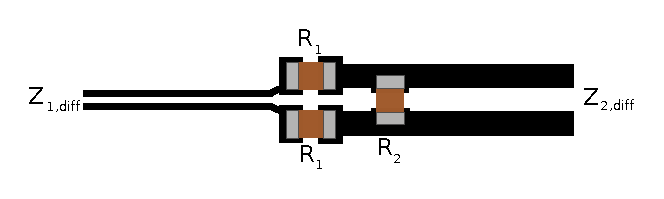
\includegraphics[width=.7\textwidth]{img/Impedmatch.pdf}
	\end{center}
	\caption{Impedance matching network. Assuming $Z_1>Z_2$, this network adjusts for properly chosen $R_1$ and $R_2$ the imedances according to requirements. The line thickness on the PCB board indicate proper matching there as well.}
	\label{fig:mpedmatch}
\end{figure}

\begin{figure}[hbtp]
	\begin{center}
	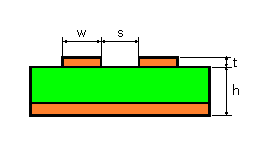
\includegraphics[width=.4\textwidth]{img/diffpair.pdf}
	\end{center}
	\caption{Sketch to define some characteristic sizes in a differential pair trace on a PCB with a potential surface below the insulator.}
	\label{fig:diffpair}
\end{figure}


\section{RTD bridge}
Current versions of the HDI have a Pt10000 RTD for measuring the temperature. A circuit proposed by Sergey Los is shown in Fig.~\ref{fig:RTDcircuit}. This circuit is included and hooked up to two ADC channels of the DTB available on the SCSI connector.

\begin{figure}[hbtp]
	\begin{center}
	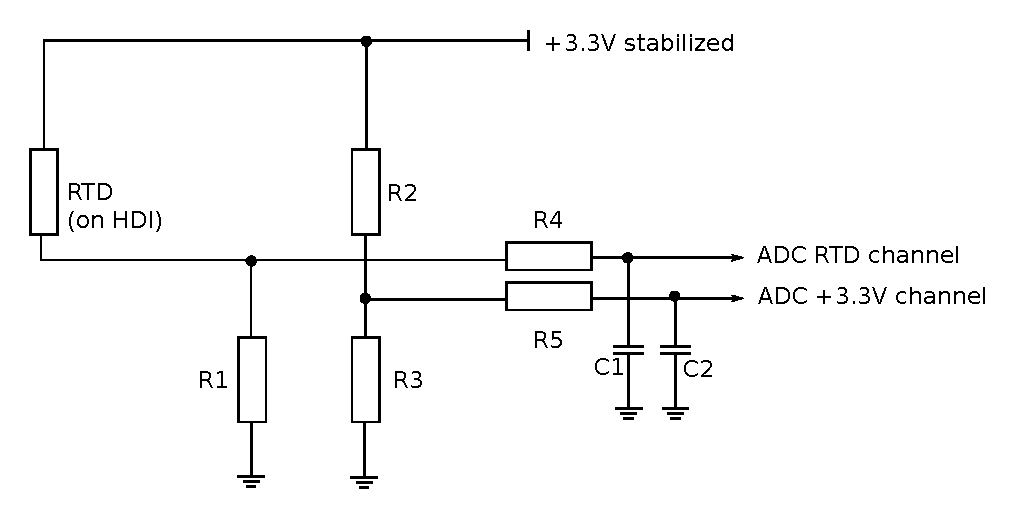
\includegraphics[width=.7\textwidth]{img/RTDcircuit.pdf}
	\end{center}
	\caption{RTD circuit. Two ADC channels are used for measuring the voltage of the RTD and 3.3\,V channel. The latter is used as a reference. The resolution is estimated to be $2\,^\circ$C.}
	\label{fig:RTDcircuit}
\end{figure}


\section{Form factor}

The size of the board are driven by the following requirements:
\begin{itemize}
    \item The PSI coldbox takes up to four modules, spaced by 60\,mm. The flex cables will therefore come out of the cold volume in the same spacing (center to center).
    \item The SCSI connectors come in a width of 64\,mm. This is wider than the spacing just mentioned. This requires to turn them by 90$^\circ$ and direct the SCSI cable perpendicular to the flex cables.
    \item The SMK connector needs to be close enough to the flex cable end, which sticks out of the cold volume by about 80\,mm.\footnote{Compared to the previous version, this is much more relaxed. This was made possible due to a reshaping of the cold plate of the box for other reasons. With this occasion, the location of the module was shifted towards the center.}
    \item The height level of the SMK connector should match the height of the insulation lid of the cold volume.
\end{itemize}
All this lead to the following specifications:
\begin{itemize}
    \item Dimension of 40 $\times$ 100\,mm$^2$
    \item No parts on the bottom side of the board
    \item SMK connector within less than 30\,mm of the edge towards the cold volume
\end{itemize}

\section{HV protection}
High voltage is supplied via the DTB\footnote{The DTB has a relay to control HV from a HV power supply and passes it via a 100\,k$\Omega$ resistor to the SCSI cable. See the DTB documentation about its HV safety.}. The following measures have been taken:
\begin{itemize}
    \item The HV is routed entirely in an inner layer.
    \item There are some spots on the board where a HV is exposed:
    \begin{enumerate}
	\item HV pin at the SCSI connector (pin 68). Accessible on the back of the board.
    
	This pin can be covered by Kapton foil, mounted by Kapton tape
	\item Two vias around the SMK connector.
    
	Can be covered with Kapton as well
	\item Four pins on the SMK connector.
    
	These pins are hard to touch if the connector is closed (which is assumes to be the standard situation when HV is on). No special protection needed. The neighbouring pins have no solder pin on the board to reduce the risk of shorts.
    \end{enumerate}
\end{itemize}

\section{Other requirements}
\begin{itemize}
    \item All differential signals should be accessible as spy pads, preferrably on the chip side for debugging. For a later version of the board, this requirements may be dropped in favour of less parasitic capacitance.
    \item In the same spirit, the power voltages and the RTD signals should be available as well.
    \item Mounting holes should be placed at appropriate locations.
    \item If tracing of TBM signals cannot be made without using vias, less important signals like the return clocks should be taken for this. In any case, vias in differential signals will be applied in pairs.
\end{itemize}


%===========================================================
\chapter{Drawings}


\begin{figure}[hbtp]
	\begin{center}
	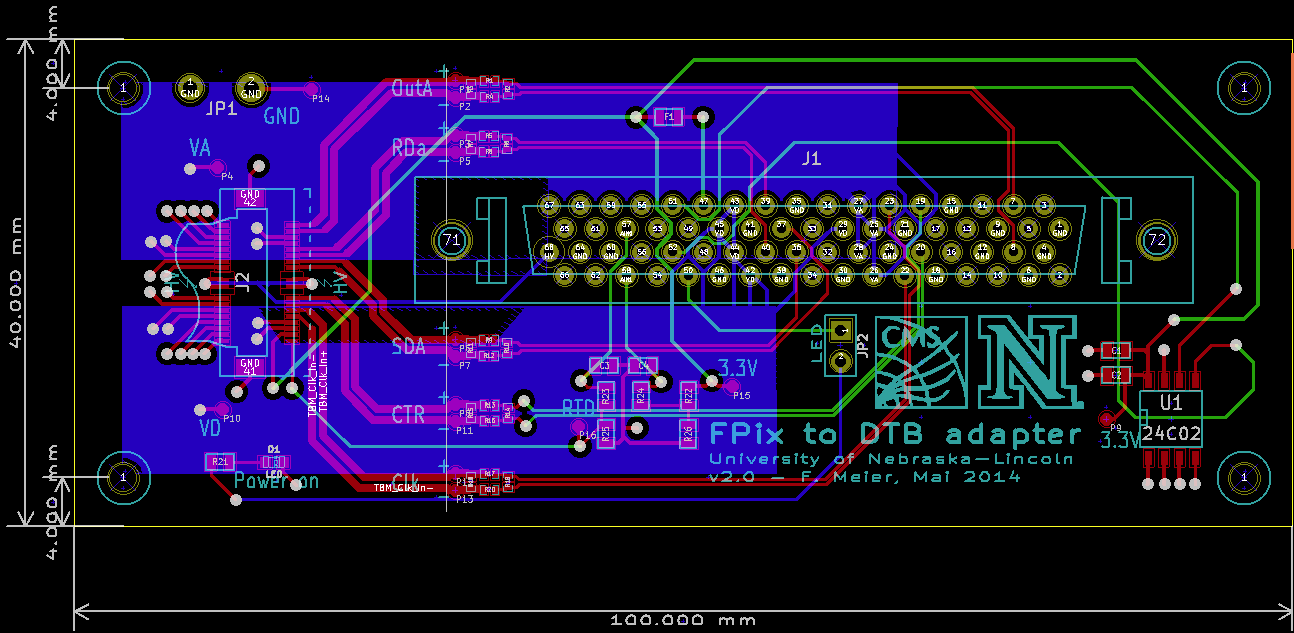
\includegraphics[width=1.0\textwidth]{img/FPix2DTBadapterDrawing.png}
	\end{center}
	\caption{Draft of a layout including some dimensions. Red traces: top layer. Light blue traces and areas: power layer. Green traces: back layer. GND plane not shown for clarity. Holes have I.D. of 2.2\,mm, good for M2 and No.\,2 screws. Mounting on a cold box is done using the four holes at the edges. Spy pads are available near the impedance matching networks and labelled for usability. Same is true for the other spy pads.}
	\label{fig:FPix2DTBadapterDrawing}
\end{figure}

\begin{figure}[hbtp]
	\begin{center}
	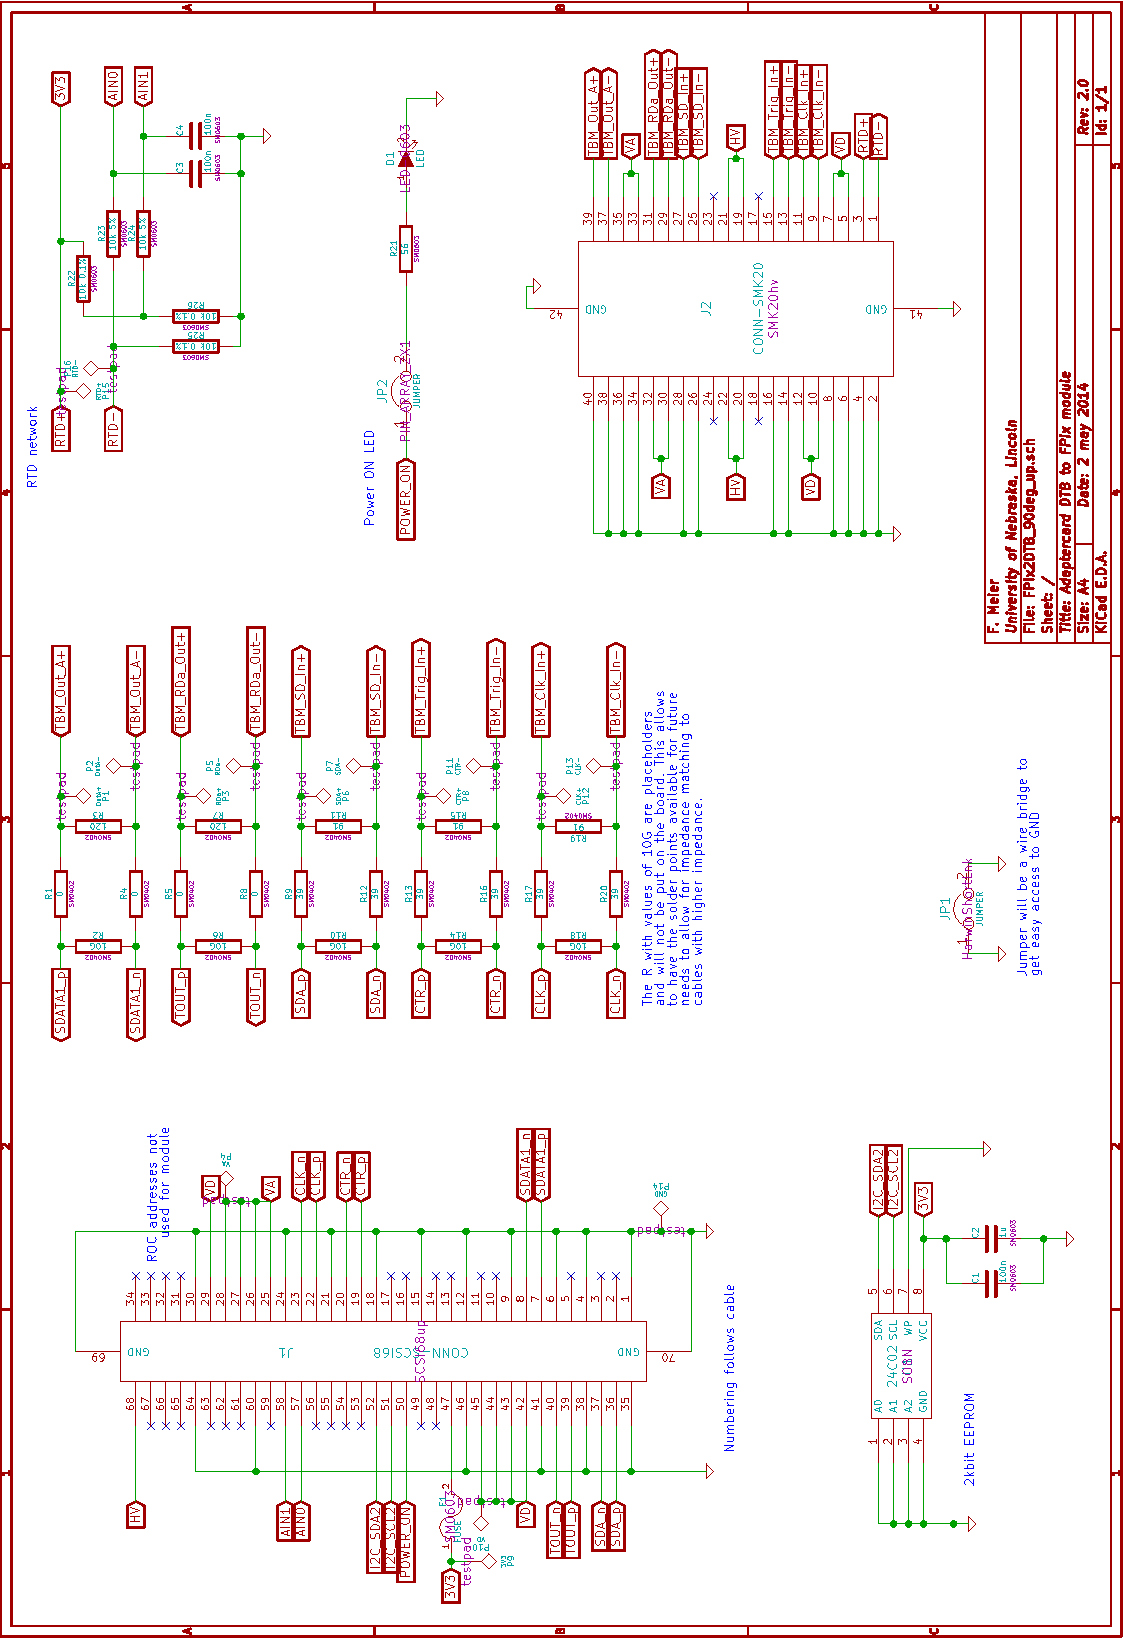
\includegraphics[width=1.0\textwidth]{img/FPix2DTB_90degSchematic.pdf}
	\end{center}
	\caption{Schematic of the circuit.}
	\label{fig:FPix2DTB_90degSchematic}
\end{figure}

\section{Bill of materials}

{\footnotesize
\begin{tabular}{cp{2.2cm}lclll}
	\toprule %-------------------------------------------------------------------------------------------------
Id & Designator                 & Package  & Quantity & Designation & Supplier & Ref \\ 
	\midrule %-------------------------------------------------------------------------------------------------
1 & C1, C3, C4                  & SM0603   &        3 &        100n & Digi-key & 1276-1011-1-ND \\ 
2 & C2                          & SM0603   &        1 &          1u & Digi-key & 587-1248-1-ND \\ 
3 & J1                          & SCSI68up &        1 & CONN-SCSI68 & Digi-key & A31826-ND \\ 
4 & J2                          & SMK20hv  &        1 &  CONN-SMK20 & SMK      & Fermilab, Sergey Los \\ 
5 & JP1                         & jumper   &        1 &      JUMPER & Digi-key & 952-1872-ND \\ 
6 & R9, R12, R13, R16, R17, R20 & SM0402   &        6 &          39 & Digi-key & P39JCT-ND \\ 
7 & R11, R15, R19               & SM0402   &        3 &          91 & Digi-key & P91JCT-ND \\ 
8 & R3, R7                      & SM0402   &        2 &         120 & Digi-key & P120JCT-ND \\ 
9 & R1, R4, R5, R8              & SM0402   &        4 &           0 & Digi-key & P0.0JCT-ND \\ 
10 & R22, R25, R26              & SM0603   &        3 &   10k 0.1\% & Digi-key & P10KDBCT-ND \\ 
11 & R23, R24                   & SM0603   &        2 &     10k 5\% & Digi-key & P10KGCT-ND \\ 
12 & R21                        & SM0603   &        1 &          56 & Digi-key & P56GCT-ND \\ 
13 & U1                         & SO8N     &        1 &       24C02 & Digi-key & AT24C02C-SSHM-T SL901CT-ND \\ 
14 & F1                         & SM0603   &        1 &     500\,mA & Digi-key & SF-0603S050-2TR-ND \\ 
15 & JP2                        & jumper   &        1 &      JUMPER & & \\ 
16 & D1                         & SM0603   &        1 &             & Digi-key & LTST-C191KRKT \\ 
	\bottomrule %-------------------------------------------------------------------------------------------------
\end{tabular}
}

\bigskip

Notes:
\begin{itemize}
    \item Do not put any resistor R2, R6, R10, R14 and R18. Leave them empty. Their space may be needed in case a cable with a higher impedance than the SCSI cable is used.
    \item The pads neighbouring the HV pads (2 on each side) are not available on the PCB. When mounting the connector make sure there is no solder under these unused pads that may create a short.
    \item Dimension of fuse F1 needs to be determined, other values are available.
    \item LED D1 can be exchanged by any other suitable type but should be of red color to match the same signal LED on the DTB.
    \item Jumper JP2 is a standard 1/10\,in jumper. Either put 2 pin plus jumper there or connect with a wire. Shipping state should be with jumper shorted, i.e. LED turned on.
\end{itemize}


